\chapter{玩偶}

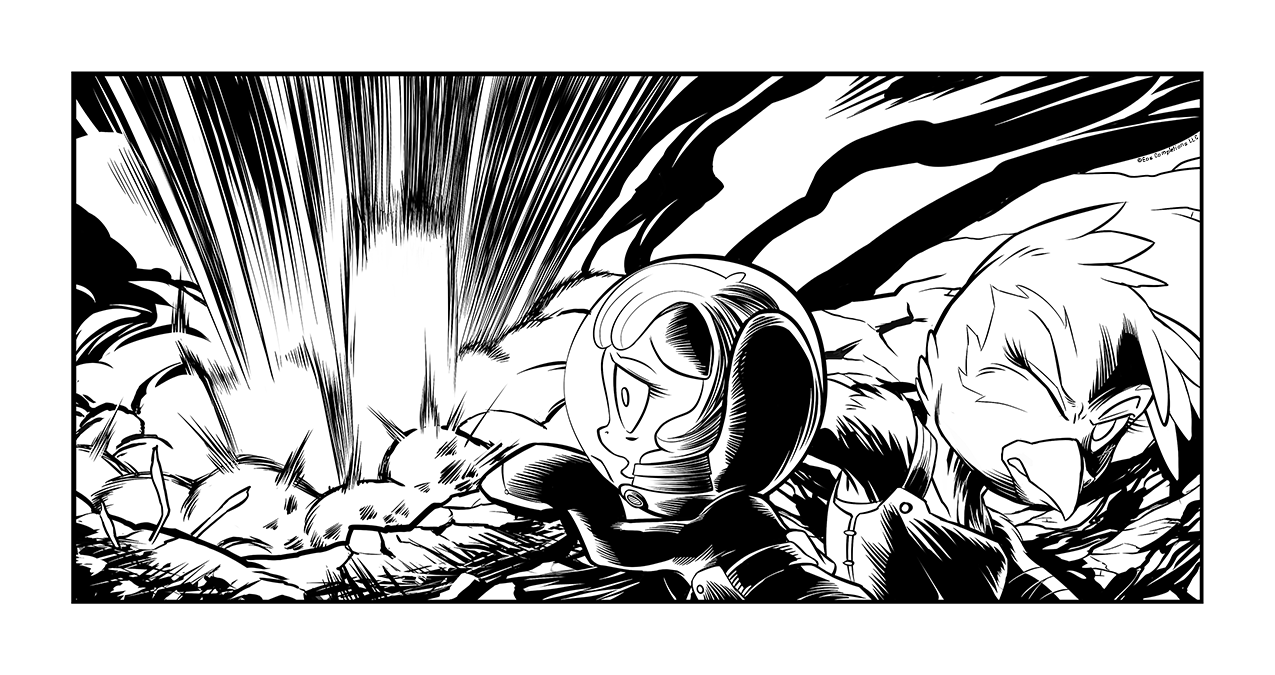
\includegraphics[width=0.9\linewidth]{image14.png}

\begin{intro}
    人生必有不可避免的阴雨日
\end{intro}

\daytimeplace{11}{22:30 PM}{小马国上空约 \SI{1800}{km} 近地轨道}{Low orbit, $\approx \SI{1800}{km}$ above Equestria}

在行星上空轨道上运行着的是普罗米修斯——一个巨大的超轻合金马造奇迹。它的形状就像一个巨大的向日葵,长长的太阳能电池板在它四周伸展着,在它的外壳上画着很多标记,比如说流星,辐射警告等等,但是最显著的还是旭日公司的标记,一个大大的天角兽,下面有一行走「可持续发展道路」的字样。

在卫星的圆形主体上,有四个巨大的圆管,长度比一列火车都要长,这些巨大的武器被金属环固定在一起。这圆管里面是被称作质子炮的武器,它使用强大的魔法电磁混合力场,是将巨大等离子团加速到近乎光速投射向超远距离目标的致命武器,每一门都有巨大的破坏力,而每一个卫星上装着四门这种「玩具」。

不过旭日公司可不是做事做一半的小马,一个这样的卫星怎么可能在需要的时候随时发射呢?所以这个卫星一共有十一个伙伴,全都零零落落地分部在小马国上空的卫星轨道组成了一个卫星网络,就像一串明亮的珍珠项链一样。而现在整个家族都将炮口指向地面,明亮的引导激光照向它们的标靶。

「{\mt ……八……七……六……}」

随着倒数计时,每一个炮管口都亮起了蓝色的电离光芒,长长的两根伸出来的磁轨就像是不详的朗基奴斯之枪,而魔力场和磁力场包围在磁轨上形成一圈圈的蓝色光环。

「{\mt ……五……四……三……}」

在卫星背后,四个舱门逐次打开,开始喷射推进剂用来抵消武器系统的巨大后坐力对轨道的影响。那些碗状的喷口之中首先是有一个红点,然后立刻像是火山口一样猛烈地喷出火焰,而前面的四个炮管已经完全被蓝色的光芒覆盖,魔力和磁力在圆环上来回流窜,随时准备释放他们的狂怒。

「{\mt ……二……一……发射!}」

\horizonline

\daytimeplace{11}{22:30 PM}{象牙塔,52号国道中段}{Ivory Tower, Big 52 SC Branch}

「{\mt 攻击确认,第一波轨道轰炸降落时间:7分钟后。}」

半数的引导激光消失了,还有一些在疯狂地摇晃着,好像是天堂发生了什么可怕的事情,但是依然有五道光柱紧紧锁定在目标上。

「为什么大家都开始撤退了?」

赫瑞塔展开翅膀,准备抓起帕比立刻飞走。

黄色的小雌驹指着基地入口说:「那里有俩没跑的,我们去问问他们?」她一边说着一边走向那守卫着大门的俩帕拉丁。

「这可不是个好点子!我的活已经干完了,我们最好跟着我们的好伙计一起跑。」

「{\mt 警告建筑物内的所有小马!你们已经被轨道轰炸瞄准!立刻离开,我们不会向你们射击,请快逃命吧!}」诘责的声音再一次在战场上回响着,然后他也跟着其他学徒和抄写员一起掉头跑。

抬起头看到那刺破夜空的红色引导激光,赫瑞惊讶地张开了喙,「你妈下的臭蛋……如果这激光只是用来瞄准的话,我可不想看它射击。」

「{\mt 警告,普罗米修斯三号,五号,十号,十一号和十二号失去信号,普罗米修斯四号和七号反推系统严重故障,普罗米修斯一号,二号,六号,八号和九号攻击完成,准备第二次,倒计时……九……八……}」

帕比皱起了眉头,声音先生从刚才开始就一刻不停的说着莫名其妙的话。这让幼驹对现在的状况更是丈二和尚摸不着头脑。面前大家都在逃命,红斗篷先生又在大叫着什么,而她的头盔上到处都是红色的警告灯。

「怎么才能把这一团乱停下来?」

「我不知道,我也不关心,我们快跑吧!」赫瑞抓起帕比伸开翅膀开始逃命。

不过马上又有个新的问题,飞行。帕比已经做好下一次飞行的准备,在下一次飞行的时候有一件事是不得不做的,是什么来着?对,是尖叫。

「咿……!别!别!不要!不要!」

「给老娘闭嘴!你丫想活命吗?」狮鹫被沉重的小雌驹拖着,完全飞不起来。

「你丫身上到底装了什么,前几天我刚让你丢了十吨的垃圾,现在你身上又都快装满了?肏!快把东西丢了,要不我们会坠机的!」

「{\mt ……二……一……第二波轰炸发射,开始准备第三波轨道轰炸。}」

「放我下来!放我下来啊啊啊啊!」帕比因为面前双蹄之间的地面距离自己太远而且移动速度太快而大声尖叫。

赫瑞塔用爪子抓着小雌驹的一只鞍带,在用力划了几次之后,终于在上面划出一个长口子。

「搞定」

「{\mt 启动修复魔法,普罗米修斯一号,二号失去信号,普罗米修斯六号,八号和十一号继续射击,倒计时……十……九……}」

物品管理系统把所有东西都固定好的同时,自动修复系统立刻补好了袋子上的大洞。

「喂,这也太诈了吧!你丫玩老娘是吧?看招!」狮鹫抓着帕比的一边把她倒了过来,这个方法看起来奏效了,因为她的包包没有扣好,小雌驹的体重迅速减轻,而身后则洒落出一长串东西,空瓶子,烂玩偶,小小的玩具车什么的。

「呀!呀!呀!不!停下!拜托放我下来!我要吓尿了!」但是这个方法同时也让帕比的飞行恐惧症更加糟糕,不过幼驹还是在「命运之石」掉出包的时候抓住了它,虽然小雌驹找到的其它好东西都已经丢了。今天真是个坏日子,而且这个蠢赫瑞塔还在欺负她。「你这个讨厌鬼!放开我!我要告诉我妈妈!」

终于帕比的体重达到一个可以承受的标准,赫瑞把小雌驹背回了背上,希望能减轻一下雌驹的惊叫声。「好了好了,已经搞定了,现在能安静坐好么,飞过那个山头我就把你放下。虽然赫瑞不知道天上会掉下什么,不过佣兵的直觉告诉他有一个掩体非常重要,虽然很奇怪到现在为止还没发生什么事情,不过一般来说,大招的蓄力时间越长威力也越大不是么?「我们现在还不能降落,帕比你不要去想飞行的事情,闭上眼睛听音乐好么?」

帕比听到之后,觉得这个音乐的主意看起来不错。

「请打开音乐!」

在下面的小马拼命逃命的时候,广播声响了起来,两个不同派系的铁骑卫现在都相信老书记官的话,迅速跑向山丘。

「{\rt 女士们,先生们,晚上好!坏孩子们还没睡觉么?孤狼的52电台给你带来新鲜的52新闻!既然我们有很多事情要讲所以我们还是先切入主题吧!}」

为什么不是音乐?为啥每次帕比打开收音机都是这个罗里吧嗦的小马在念?帕比想要音乐!而现在地面已经是一个快速划过的残影,而声音先生也在唠叨着什么奇怪的东西。帕比想要哭,而在防护服的背景音之中,声音还提示着剩下的三个卫星依然在继续攻击。

「{\rt 首先是第一条:南岸的事情开始变得一团糟,看起来土匪又在铁毡附近的路上出没,不过这一次他们看起来比之前装备更加精良也更加有组织,或许他们有了新的领导?这只表示将来会有更多更大的麻烦。如果你们在花椰菜镇南边的纪念碑和铁毡镇之间旅行的话,千万要小心,而且避免走通向翠绿海滨的路,沿着大路赶快赶路,小心驶得万年船!}」

狮鹫快速地飞过夜空,轻松飞跃那些还在逃跑的小马,虽然她还不太明白为什么所有小马都在逃命,不过赫瑞还是背着快把她勒死的帕比快速飞离。

「{\rt 而且祸不单行的是,我们还收到另一条来自NCA的政令,高兴么?NCA现在认为每个旅行商都是土匪,他们开始逮捕旅行商,如果你计划往那边走的话,建议你重新考虑一下是否需要去岩块城或者通道镇来做买卖,毕竟现在52号国道北边还算安全。}」

赫瑞塔降落在山坡背后,大口地喘着气,帕比一看到坚实的地面就立刻从她背上跳了下来,对那个坏小鸡吐着舌头,「哼!为啥老是欺负我!我还是你朋友呢!」

「滚边去死丫头……」赫瑞上气不接下气地说:「老娘才没欺负你,那边不知道要发生什么……发生什么很糟的事情。」

「{\rt 然后是最后一个新闻,看起来一个老商人从他长长的路途回来了,他四年之前带着一个双头牛拉着整车的垃圾出发,而回来的时候带着……好吧……还是一个双头牛和整车的垃圾,还有一箩筐的故事,或许改天我可以和你们讲讲他所拜访的那些城市。他说远处在河的对岸有一个灯火通明的大城市,还在河上建了一个大坝来发电……哇哦,或许我们这里可以考虑建一个\footnote{\emph{FoE: PH} 的剧情}?好了,晚间新闻播报到这里,来点音乐吧!}」

帕比好奇地歪着头,「发生什么坏事?但是我妈妈在那里!」幼驹转向象牙塔,现在那个建筑已经在几公里之外,被红色的引导激光微微笼罩上一层诡异的颜色,于此同时它上面的云层忽然变得明亮。

这个时候收音机开始播放音乐了。

\begin{music}
雨滴不断落在我鬃毛上

\begin{englishlyric}
    Raindrops keep falling on my mane,
\end{englishlyric}

\medskip

就像是一个幼驹没有可爱标记

\begin{englishlyric}
    And just like the foal whose cutie mark is not there,
\end{englishlyric}

\medskip

什么事都不顺利

\begin{englishlyric}
    Nothing seems to fit there.
\end{englishlyric}
\end{music}

纯白的光之长枪穿破云层,径直刺向红色的靶心,那些光束重重地砸在白色的象牙塔上,冲击的力道就连站在这么远赫瑞塔都感受得到。

\begin{music}
雨滴不停落在我鬃毛上

\begin{englishlyric}
    Raindrops are falling on my mane.
\end{englishlyric}

\medskip

雨不停的下——

\begin{englishlyric}
    They keep falling---
\end{englishlyric}
\end{music}

被击中的建筑物首先是被一道纯白的光芒所包裹,然后建筑的外墙似乎膨胀了一些,看起来就像是气球做的一样,有那么一瞬间那象牙塔看起来就像是要飘起来一样,但是下一瞬间它就炸成了无数的碎片——墙,窗户,大门……就像是妈妈给她看的某个展示房间零件的滑稽画册,接下来那些零件开始四散飞去。一块块外墙就像纸片一样被炸飞上天,整个象牙塔看起来就像是个纸片城堡一样被炸得四分五裂。

在这之后声音才传来,帕比一开始听到的是一阵尖锐的呼啸声,就像是用蹄子在玻璃上划发出的声音一样,在长长的呼啸声之后就是轰隆的巨响,不过不仅仅是一个「轰隆」,而是持续不断的轰隆声,就像是滚滚天雷一般。

帕比希望妈妈能在这里和她一起看这幅景象,真是太有趣了!不对……等等……妈妈在……妈妈应该在哪个漂亮的白色建……哦不!

小雌驹瞪大眼睛举起蹄子指向曾经是象牙塔的地方,她的表情被惊恐所覆盖。

「妈妈?」


\begin{music}
    所以我和太阳公公讲理
    

\begin{englishlyric}
    So I just did me some talking with the sun,
\end{englishlyric}
    
    \medskip

    我不喜欢它的做法
    

\begin{englishlyric}
    And I said I didn't like the way she got things done.
\end{englishlyric}
    
    \medskip

    因为它没有认真做事
    

\begin{englishlyric}
    She's sleeping on the job.
\end{englishlyric}
\end{music}

「{\mt 警告,普罗米修斯六号弹药已用尽,其它卫星信号丢失,攻击停止,目标区域将会在15分钟之后恢复安全。感谢您选择旭日科技作为您的主要火力覆盖武器。旭日科技——走可持续发展道路。}」

% NOTE: try the alternative. ???

帕比目不转睛地看着那白色的光点穿过云层不断落在她的任务目标上。为什么还不停下来?什么时候才会结束?那东西已经弄出很大噪音了,应该停止了,不是么?如果只是一下下烟火的话还算有趣,但是现在有点……可怕。帕比屏住呼吸,拼命祈祷着,希望每一个落下来的光线都是最后一道,但是马银色的光雨却违背她意志不停地落下。继续蹂躏着声音先生说的妈妈缩在的地方。

不过……等等!那个箭头,那个箭头还在!希望还在!帕比欢呼着,没有什么可以阻止妈妈,知道厉害了么光雨!


\begin{music}
    雨滴不停落在我鬃毛上
    

\begin{englishlyric}
    Those raindrops are dropping on my mane.
\end{englishlyric}
    
    \medskip

    雨不停的下——
    

\begin{englishlyric}
    They keep falling---
\end{englishlyric}
\end{music}

另一波光雨就像是流星一般穿过云层砸在废墟之上,这一次似乎击中了研究中心的发电厂,因为这一次冲击伴随着一个巨大的绿色火球并且腾起高高的蘑菇云直冲天空。

「{\mt 警告,检测到微量辐射,威胁等级:可忽略。}」

罗盘上粉色的箭头闪烁了三次然后消失了。帕比等待着它再一次出现,希望它再一次出现,祈祷着它再一次出现!但是罗盘还是空空如他,防护服只是通知她任务『追雨』已经完成。

为什么那些银色的东西还在落下?已经结束了,全都结束了……箭头没了,妈妈没了!妈妈……已经没了?不……不可能!妈妈还……妈妈一定还在箭头指的地方……但是……但是现在箭头也不见了!帕比一直跟着箭头,因为那个箭头指着妈妈在的地方,但是现在箭头不在了,再也没有地方可以去,再也没有什么东西剩下……只剩下一堆坠落的繁星……在离开中心城的第一次,小雌驹不知道该做什么。

妈妈不在了。


\begin{music}
    但是我只知道
    

\begin{englishlyric}
    But there's one thing I know.
\end{englishlyric}
    
    \medskip

    那些从天而落的忧郁
    

\begin{englishlyric}
    The blues they sent to meet me,
\end{englishlyric}
    
    \medskip

    绝对不会打败我
    

\begin{englishlyric}
    Won't defeat me.
\end{englishlyric}
\end{music}

帕比大睁着眼睛,幼驹完全不动了,空洞的眼睛看着前方,脸上露出惊讶的表情。

赫瑞塔拍着小马的肩膀,想要在隆隆的爆炸声之中说点什么,不管天上落下来的是什么,现在地面上估计已经什么都不剩下了,但是就算刚刚发电机的爆炸之后,那些炮弹还在不停地落下来,那些家伙只是在浪费弹药而已。

「别担心!你的妈妈不在那!我去里面看过!她不在象牙塔!」

但是帕比没有反应,小雌驹甚至没有听进去一个字,赫瑞用力摇着她,但是小雌驹没有一丝反应,只是像一个坏掉的玩偶一样,脑袋在头盔里面晃来晃去。


\begin{music}
    没有什么值得让我伤心
    
    
\begin{englishlyric}
    It won't be long till happiness steps up to greet me.
\end{englishlyric}
\end{music}

「别这样帕比!你经历过比这糟糕得多的事情,喂喂,有在听我说话么?」赫瑞戳了戳小雌驹,只是让她的头像摇头娃娃一样晃来晃去。「怎么回事?醒来啊!」但是还没有反应。

「我们赶紧离这里远点,最后那爆炸把放射性尘埃喷得到处都是,」年轻的佣兵无力地叹息着,「为啥是我!我只是接受个简单的工作而已,为啥每一次我想干点儿啥事都要去南边!好吧,我才不想知道为啥!」赫瑞把帕比背在她背上,急忙想追上铁骑卫。

「不管怎么说,那些家伙还差我一半工钱,我们走帕比!」狮鹫慢慢地走着,总是觉得不对劲,「我可受不了你这个样子,说点话好么?」还是没反应。

「好吧,你想要我来硬的?那么我来硬的!」赫瑞塔抓起帕比的一个蹄子晃着,捏起嗓子学着她朋友那聒噪的音量,「好啊!我们走,漂漂坏狮鹫!」

不过看起来攻势开始慢慢减弱,只剩下零星的几道光线穿过云层落在地面上。

「真棒,现在我在和一个大木偶聊天……老娘真他么开心……」

\horizonline

\daytimeplace{12}{4:30 AM}{铁骑卫前哨站,52号国道中段}{Steel Ranger's Outpost, Big 52 SC Branch}

一队铁骑卫,包括书记官还有侍从驻扎在上脚下的一个营地,他们正在从建设在山内部的一个碉堡里面搬出各种箱子。

这个小小的碉堡在战前曾经是一个观测站。而在一个世纪之前这里就成为了铁骑卫的前哨。整个建筑建设在山内部,顶部还有个高高的观测塔楼,不过里面的空间只能容纳一个排的士兵,虽然这个设施很小,但是作为铁骑卫存放补给物资的地方是再好不过。

「你看,事态明显已经超出预期,我现在真的是一个子儿都没有了。」招呼赫瑞塔的冷浴忙得都没时间脱下头盔。

狮鹫轻蔑地哼了一声,「老娘干了活了,他们的发电机和内部防御系统都已经干掉了,不管那基地是不是给流星砸了,老娘现在就要赏金!」

「你可以去那弹坑里面找你的赏金去,想拿什么拿什么,我现在还有个营地要建设,还有一大堆杂事还有一堆俘虏,别给我添乱了好么!」帕拉丁说着头也不回地走开了。

赫瑞塔举起帕比的蹄子,指着帕拉丁学着他的声音说:「你个大坏马!你这是在作弊!不要说些不明觉厉的话,按约定给钱好么!」

冷浴听到这个声音定住了,然后转头看着像玩玩偶一样抱着幼驹的狮鹫,「你知道么,你这么做很诡异的。」

「不要觉得你比人家聪明!我不笨!乖乖地给我朋友钱!」狮鹫戳了戳帕比的头盔,让帕比的脑袋转向她的方向,这个动作让帕拉丁尾巴毛都竖起来了。

「别玩了好么!我说,我很抱歉你朋友发生的事情,但是我们有自己的麻烦!」冷浴不知道哪一点更可怕,是刚刚活蹦乱跳的小雌驹现在就变成这个呆呆的样子,还是那个年轻母狮鹫把她当做一个求钱玩偶。

赫瑞塔让帕比双蹄交叉,然后转过她的头,「哼!人家不想当你的朋友了!」

「好吧好吧!我投降!我们现在还要处理那些投降的铁骑卫,然后我派诘责书记官看看能帮快乐帕比什么忙,最后我在看看箱子底能不能翻出点东西当做给你的报酬好么?」

帕比晃着蹄子,「耶!」

「而且别玩儿那幼驹了,有够可怕!」帕拉丁不等狮鹫回话赶紧走开了。

赫瑞呆立在那里,脸上带着傻笑看着铁骑卫离开,然后慢慢地走开,直到那个营地离开到视野之外。然后重重叹了口气,抱着小雌驹说,

「别担心,我们可以搞定一切问题,别……别走……好么?」

狮鹫紧紧抱着帕比小声地说:「我知道我并不算是个好朋友,但是我真的不想欺负你,只是想和你开个玩笑……你知道当个佣兵有多难么?你当然不知道。你……你只是到处玩儿的不死幽灵,什么事情对于你来说都好轻松,我真的很嫉妒你,而且我非常讨厌你,因为你就算一个马呆着也不会寂寞,但是我孤单得要死。」

诘责书记官这个时候走了过来,「喂,火红小姐,冷浴在那边的碉堡里面找你。」老独角兽站在那里等她回答。

赫瑞吃惊地跳起来,拼命想把黄色小马放到她身后,「等!等一下!」

「好的……」书记点点头。

狮鹫一脸又惊又怕的表情问:「你刚刚看到什么了吗?」

「没,我没有看见你抱着你的朋友哭。」

赫瑞看起来放松了一些「很好。」半狮子说着站了起来,然后戳着诘责的肩膀说:「帮我看好那个累赘。」她顿了顿,对上老书记官的视线之后,她马上就败下阵来。

「拜托你了……」

「没问题,实际上我正在到处找她……你先忙。」诘责等赫瑞塔走开之后走向那个呆呆站在那里神游天外的小雌驹。

「我又来了,我们又见面了……介意我看看你的包么,不介意么,好。」书记官表情严肃地打开帕比的鞍包,在里面翻找着。「不管怎么说,你也翻过我的口袋,所以这也算是以牙还牙,我看看你都有些什么?」

% \thpr{坏掉的玩具……彩色玻璃碎片……灯泡……瓶盖……我的另一半眼镜……}

% TODO: 这是什么鬼溢出?
% NOTE: 修改译文(去除一个「的」)来解决

\thpr{坏掉的玩具……彩色玻璃碎片……灯泡……瓶盖……我另一半眼镜……}


啪嗒!

\thpr{……哪里来的恶心声音?}

独角兽把他的蹄子抽出包裹,看着上面裹着的一层绿色粘液皱起眉头,「看在露娜的份上,这是什么怪味?」诘责又戴上一副橡胶蹄套,小心地检查里面是什么东西漏出的粘液。「一个死肉食灵?为啥这幼驹要带着一个死肉食灵?」

\thpr{等等……肉食灵尸体……一个不死小雌驹……这个……是她的宠物么?这真是个伤心的故事……{}}

书记官把那尸体放回袋子里面,然后检查另一个包,为什么她把所有东西都放在一个包里面,另一个包包基本是空的呢?

在快速检查了一下第二个包之后,诘责找到了他要找的东西,他吹着口哨把那个东西拿了出来。

「这就是鬼牌么……旭日科技,这一切就说得通了。」老独角兽打了一个响鼻,在他的哔哔小马上检查着这个武器,「天使之瞳……普罗米修斯系统……来自天空的制裁,还真是贴切。」

诘责看着远处,和小雌驹目光差不多相同的方向,然后说:「我这回欠你的情可真不好还,如果不是你用轨道轰炸阻止了那场战争,不知道多少年轻小马会死在这场愚蠢的斗争中。你从天上召唤的流星雨拯救了双方的生命。」

书记官轻抚着帕比的头盔,「这场战争太过可笑,兄弟阋墙,生灵涂炭。而长老只关心他们的利益。小小的连长都知道关心他手下的士兵,而我们的那些大角色呢……那群老顽固就知道数着蹄上的瓶盖和蹄下的士兵,完全不管那些士兵的死活。」

诘责叹了口气再一次拍拍帕比的背,「我想我会帮你保守这个小秘密,天使之瞳,我原谅你摧毁我的……几乎大半生的劳动成果。」他嘴角微微向上弯起,「留下了我最珍贵的东西——我的学生们。」

独角兽再一次叹气,感受到自己似乎一瞬间就变老了,但是不知道为什么现在他却很开心,他已经不记得上一次感受到如此如释重负的快乐是什么时候了。「不管怎么说,52号国道有所取,有所给。我给你一些东西换你的玩具吧。」

诘责把天琴的玩偶放在帕比的包包里面。「给你,和她做个好朋友,别给她染毛好么?看着你我也很想要个孙女了,可惜我的儿子……算了,不提也罢。」

独角兽站起来,留下帕比独自坐在山丘之上。

「哦,还有一件事,南边有个小镇叫花椰菜镇,不过在很久之前那里还不叫这个名字的时候,那边只是个农场,小马们叫那里阴雨营地,而且那里的集会大厅现在还叫阴雨·黛丝……你最好亲自去看看。」

老马说完这几句话之后,消失在山丘之后。

「{\mt 任务日志更新,接受新任务:南方风暴,花椰菜镇大厅定为主要任务目标,花椰菜镇大厅位置已经标注在罗盘上。}」

一个粉色的箭头开始闪光。

\horizonline

\daytimeplace{12}{5:00 AM}{铁骑卫前哨站,52号国道中段}{Steel Ranger's Outpost, Big 52 SC Branch}

坐在碉堡里面的冷浴看到赫瑞塔进来之后,对她点了点头,「很抱歉这么快又叫你,不过我想到个点子解决你的报酬,还有我的麻烦。」

赫瑞塔没有立刻回答,而是慢悠悠地走进物资当中,这个碉堡里面空间很狭窄,天花板也很低。到处乱堆的各种箱子加剧了这种空间的狭窄感。除了那些不长蹄子的垃圾和长蹄子的垃圾之外,赫瑞塔注意到这里还有个梯子,似乎是通向上方的瞭望塔。

在这个狭窄的空间里面挤着七个小马,两个穿着标准的动力装甲,因为他们没带头盔所以赫瑞塔认出来他们是高斯和冷浴,另外五个对于赫瑞塔来说是新面孔。他们被铁链拷在一起,脸上带着惊恐和愤怒以及耻辱混杂的表情。看着那几张臭脸赫瑞塔就知道那个帕拉丁接下来不会说什么好事

「我深表怀疑。」

冷浴不管那佣兵的吐槽,接下来继续说:「这些铁骑卫依然忠于他们的长老,不过现在基地完全灰飞烟灭了,他们也不想加入我们,所以他们需要护送穿过沙漠到通道镇,所以我现在需要一个有空中侦察能力的雇佣兵,我想你是最适合的。」

赫瑞塔轻蔑的哼了一声,「你丫是不是觉得老娘是给你当保姆的?我还有我的事要忙,你还欠我瓶盖!」

「我知道,所以我向你提出这个计划,我们帮你看好帕比,看看能不能想个办法让她说话,或许我们可以想点别的办法。我想你对于她现在的状态一点辙都没有,而且我会给你武器和弹药,还有瓶盖,怎么样?」

就是送这几个蠢货过沙漠就能去帮帕比的忙并且赚几个瓶盖外快?听起来不错的样子。

「你丫又在耍什么花枪?」

帕拉丁皱起眉头,「我才没想骗你!我只是想你把事干好,我烦死校对合同上的每一个标点符号位置了!算我求你好么,如果你不这个干的话,我只好把这些俘虏全部处死了。」

听到这句话,一个年轻雌驹吓了一跳,「等等……我们已经投降了!根据条例你不能做那种事情!」另一个小马,一个脸上带伤疤的雌驹用蹄子拍了她后脑一下叫她闭嘴。

% TODO: 标点问题

「闭嘴,你还想要啥,给你端杯茶然后跪下来道歉?」另外三个囚犯只是低头沉默不语,但是那个年轻雌驹又继续说。

「诘责书记官绝对不会允许那种事情发生!我可是他的得意门生!我……」

砰!

整个房间安静了下来,每一对眼睛都盯着高斯还在冒烟的枪管,那个年轻雌驹大气不敢出,更别说去回头看她脑袋边墙上的子弹坑,整匹马抖的和筛糠一样。

「闭嘴!」

高斯的声音让那年轻的雌驹用蹄子掩着嘴无声地哭泣着,而其他士兵一脸轻蔑的表情看着她,尤其是那个带伤疤的雌驹,比起高斯刚才做的事情,那个学徒懦弱的表现。

高斯转过头接下冷浴的话茬,「我们只是做我们该做的事情,狮鹫,冷浴和诘责想要和平解决这件事情,但是不是所有小马都喜欢这个样子,所以,你打算怎么办?」

年轻的雌驹还在那低声地哭着『我不想死』什么的。

赫瑞直视着高斯的双眸,然后又看看那五个囚犯,努力忽略坐地上那雌驹身体下面正在慢慢扩大的一滩淡黄色液体。

老娘去你妈逼的!

\thpr{所有小马都是漂漂马,漂你娘下的蛋,这次是为了帕比,为了帕比才做这破事。}

「好吧好吧,你赢了!我护送他们到北边去,如果我回来的时候帕比不在这里,你丫最好咬紧牙关,老娘会把你的每一颗牙都打出来,帕拉丁机械战警,老娘有翅膀有枪,你别以为你跑得掉!听懂了没有?」

而帕拉丁则一副似笑非笑的表情面对着狮鹫点了点头。

「现在我去和那个什么诘责聊聊,确保他不会对我朋友做什么奇怪的事,你丫最好让这五个在我回来前做好出发准备。

狮鹫像个公主一样趾高气昂的走出碉堡。

她一走出去高斯就不屑地说:「就她这幅中二德行,还自称佣兵?」

「不管怎么说,我们还是需要她帮忙,干得好高斯,刚才那虚张声势彻底把她唬住了……」

「我没说假话……」

「高斯,你别吓我好么……」

\horizonline

\daytimeplace{12}{5:30 AM}{铁骑卫前哨站,52号国道中段}{Steel Ranger's Outpost, Big 52 SC Branch}

「你说她走了是什么意思?她不是和那红马在一起么?诘责?诘责你丫给老娘滚出来!」赫瑞塔彻底发飙了,她只是走开一会儿去和铁骑卫谈话,然后帕比就不见了,「我……我简直不敢相信!你在开玩笑是不是,她一会儿就会从哪个角落里面叫着『惊喜』跳出来是不是?我看起来像个傻瓜么?像么?像么?」

年轻的侍卫被狮鹫追得步步后退,「我……我也不清楚,诘责书记官出去散步了,还没回来……」

「好吧,那么他是不是带着一个小孩子?」

「我……我不清楚……等等……他回来了!你找他吧!我有事,失失失失陪了!」年轻的士兵趁赫瑞塔主意老独角兽的时候一溜烟逃走了。

诘责走进营地,回头看了一眼地平线,「希望最终有一年你能找到幸福,小家……」红斗篷小马转过身就刚好和狮鹫布满血丝的双眸对上了。「哦,你这么快就回来了。」

「对,老娘回来了,帕比呢?」佣兵怒嚎着。

「别担心,她现在很好,你接受冷浴的任务了?」

赫瑞点点头,但是看起来还是很失落的样子,「当然,不过我走之前想看看帕比。」

书记官微笑着看着狮鹫的双眸,「没有必要去看那个小家伙,她不会有事的,你信我的,去帮那五个小马吧,他们比帕比更需要你的帮助,至少现在是。」

看着那双深邃而又睿智的双眸,如此的……有魅力……帕比会没事的,既然书记这么说了,对吧?

「我……我想说啥来着?」

「既然忘记了就说明没啥重要的,你看,帕拉丁高斯在那里等你,你准备好之后去和他说吧,」书记官笑了笑,对于这样头脑简单的家伙,这种催眠术是在是百试不爽。

高斯从碉堡里面带着五个小马走了出来,现在他们已经解开了镣铐,「火红女士,队伍已经准备好了!」

狮鹫走到帕拉丁面前,想要说些什么,但是马上看到那堆战俘的打扮,「我说,他们连个烧火棍都没有我怎么护送他们穿过沙漠?」

「我不知道,你可以给他们你的装备……或者去铁锈庄园买点,祝你好运铁娘子。」虽然他带着面具看不到表情,不过声音上就可以听出来他玩的很开心。

赫瑞塔耸了耸肩,「哼,老娘自个儿也搞得定……你丫看好帕比就是了,阿杰铁卫机械战马。」

「你再叫一次……」

「你最好习惯这个名字。」狮鹫回过头去对那五匹马挥了挥爪子,「来吧,出发吧,老娘在这个臭烘烘的马厩一刻也呆不下去了」狮鹫带着那几个马向北方走去。

\horizonline

{\rt 听众朋友们!大家好!今天早上给你们带来了爆炸性的新闻!绝对是爆!炸!性的!蝴蝶小雌驹23告诉我昨晚在铁锈庄园南边有一个漂亮的灯光魔法秀,就在象牙塔的方向,我虽然不知道具体细节,不过看起来有谁用超大号大炮轰击了那里,因为几公里开外都可以看得到,整场战斗貌似持续了不到半小时,绝对是我们见过最大的爆炸……好吧,不算岩块城的那个大爆炸……不管怎么说,我不知道是谁炮击了谁为了什么,但是如果没什么事情的话你最好避开象牙塔附近。

然后是坏消息,一个失去联络车队在铁毡附近被找到了,那里躺着至少八个卫兵还有商人一家子的尸体,那群强盗现在变得更加猖獗了,旅行者们你们最好结伴出行,并且尽量避开南边。

最后,是给那些迷失在路途找不到家的小马们一首歌,希望星空引导你们,请听马库斯小马带来的歌曲。}


\begin{music}
    千里之外我可以看到那明星
    

\begin{englishlyric}
    I can see that lone star from a thousand miles away,
\end{englishlyric}
    
    \medskip

    它在呼唤我回家
    

\begin{englishlyric}
    Calling me back home, though I ventured far astray.
\end{englishlyric}
    
    \medskip

    明星照耀我回家之途
    

\begin{englishlyric}
    When I see that beacon shine, and call me all alone,
\end{englishlyric}
    
    \medskip

    呼唤我回到甜蜜的小马国
    
    
\begin{englishlyric}
    It calls me back to Equestria and a home.
\end{englishlyric}
\end{music}

\horizonline

\daytimeplace{12}{9:30 AM}{花椰菜北方,52号国道南段}{North of Broccoli, Big 52 S Branch}

黄色的小雌驹踩着红色滑板飞驰在52号国道上,紧紧跟随着那个粉色箭头的方向。

「我就知道妈妈没有事,我是说……我只是有点……嗯……累了!对,累了,别担心!而且那怕音姐姐一直在我耳边吧啦吧啦的罗里吧嗦,我是说……我去,谁想要翅膀啊?」帕比喋喋不休得讲着,也只有自律智能可可以忍受这种话唠。

「你知道最可怕的是什么吗?我记得下银雨的时候睡着了,但是我醒来的时候完全在另一个地方!难道我会梦游?嘿,声音先生,你在听么?」

「{\mt 肯定,语音交互界面一切正常。}」

「很好,我很奇怪赫瑞又去哪儿了,她总是一回头就不见了……好吧,或许她在下一座城镇,那里叫什么来着?」

「{\mt 花椰菜}」

「呃,我讨厌花椰菜!我和你说过吗?」

「{\mt 四十八次。}」

「好吧,我真的真的真的很讨厌它们!我希望妈妈不是去那里买花椰菜的,我可不想大老远跑到那里然后吃花椰菜馅饼!」

在远处,一个破旧的路牌竖立在路边写着52国道南段入口,不知道是谁在下面加了一行字。

\begin{center}
    花椰菜镇,12公里。
\end{center}

~\vfill

\begin{note}
    升级(Lv 13)

    新技能解锁:专业忠诚——等等帕比,不是这个样子的,我来帮你……在你进行爆破,开锁,医疗,修理,科技,生存鉴定的时候,你可以用同伴的技能来代替你的技能做鉴定,同时开启新的对话选项。
\end{note}



